\documentclass{article}
\usepackage{geometry}[margin = 1inch]

\usepackage[utf8]{inputenc} % allow utf-8 input
\usepackage[T1]{fontenc}    % use 8-bit T1 fonts
\usepackage{hyperref}       % hyperlinks
\usepackage{url}            % simple URL typesetting
\usepackage{booktabs}       % professional-quality tables
\usepackage{amsfonts}       % blackboard math symbols
\usepackage{nicefrac}       % compact symbols for 1/2, etc.
\usepackage{microtype}      % microtypography
\usepackage{enumerate}
\usepackage{graphicx, xcolor, ulem}
\usepackage{algorithm,algpseudocode}
\usepackage{multirow}
\usepackage{bbm}

\usepackage{amsmath,amsfonts,latexsym,amssymb,amsbsy, amsthm}
\newcommand{\mb}[1]{\boldsymbol{#1}}
\usepackage{footnote}
\usepackage{thmtools, thm-restate}
\usepackage{soul}
\newcommand \seb[1] {{\color{red}#1}}
\newcommand \sg[1] {{\color{red}(Swati: #1)}}
\newcommand \hm[1] {{\color{red}(Hassan: #1)}}
\newcommand \sge[1] {{\color{red}#1}}
\newcommand \hme[1] {{\color{black}#1}}

\newtheorem{theorem}{Theorem}
\newtheorem{proposition}{Proposition}
\newtheorem{lemma}{Lemma}
\newtheorem{corollary}{Corollary}
\newtheorem{definition}{Definition}
\newtheorem{claim}{Claim}
\newcommand{\ba}{\ensuremath{\mathbf{a}}}
\newcommand{\x}{\ensuremath{\mathbf{x}}}
\newcommand{\bd}{\ensuremath{\mathbf{d}}}
\newcommand{\y}{\ensuremath{\mathbf{y}}}
\newcommand{\bv}{\ensuremath{\mathbf{v}}}
\newcommand{\A}{\ensuremath{\mathbf{A}}}
\newcommand{\bmu}{\mb{\mu}}
\newcommand{\blam}{\mb{\lambda}}

\DeclareMathOperator*{\argmin}{arg\,min}
\DeclareMathOperator*{\argmax}{arg\,max}
\DeclareMathOperator*{\Argmin}{Arg\,min}

\newcommand{\state}{\Statex  \hspace*{\algorithmicindent}\hspace*{\algorithmicindent}}
\newcommand{\statex}{\Statex  \hspace*{\algorithmicindent} \hspace*{\algorithmicindent}\hspace*{\algorithmicindent}}

\algnewcommand\INPUT{\item[{\textbf{Input:}}]}
\algnewcommand\RETURN{\item[{\textbf{Return:}}]}

\newtheorem{innercustomthm}{Theorem}
\newenvironment{customthm}[1]
  {\renewcommand\theinnercustomthm{#1}\innercustomthm}
  {\endinnercustomthm}


\allowdisplaybreaks % To allow page breaks inside equation environment
\interdisplaylinepenalty=2500 % allows page breaks within

\newcommand{\innerprod}[2]{\left \langle #1,  #2 \right \rangle}
\newcommand{\innerprodu}[2]{ \langle #1,  #2 \rangle}

\begin{document}

\subsection*{Notation}

The ground set is denoted by $N$, and $n = |N|$. A \emph{random} or \emph{randomly generated} point (unless specified otherwise) is $(x_1, \ldots, x_n)$ where $x_i = |y_i|$, and $y_i \sim \mathcal{N}(0, 3)$ and random variables $y_i$ are i.i.d. By \emph{close points} $x, y$, we mean that $y = x + \mathcal{N}(0, \sigma I_n)$, where $\sigma = \frac{1}{n^2}$ for now. We'll later vary $\sigma$. By close points $x_0, \ldots, x_k$, we mean that $x_0, x_i$ are close points for each $1 \le i \le k$, and $x_i - x_0$ and $x_j - x_0$ are independent for $i \neq j$.

\subsection*{Iterates for close points}

\begin{figure}[h]
    \centering
    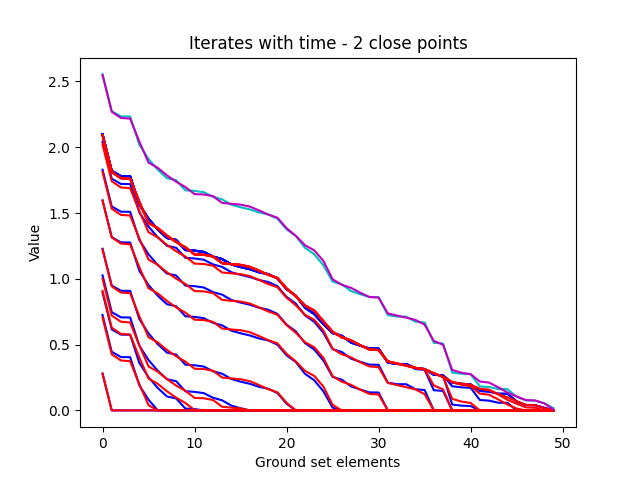
\includegraphics[width=0.43\textwidth]{code/figures/50-close-points-iterates.png}
    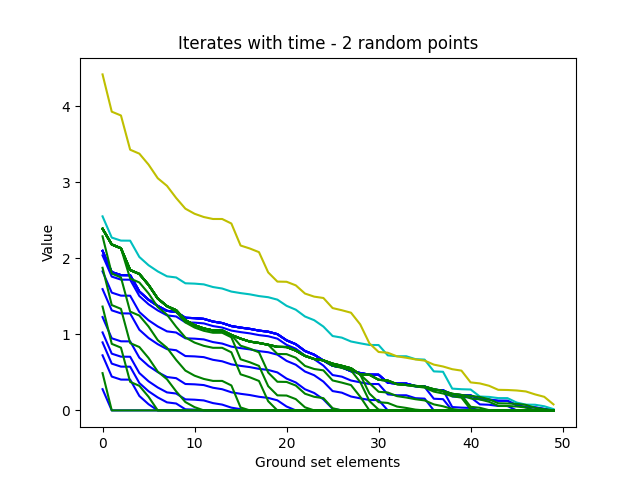
\includegraphics[width=0.43\textwidth]{code/figures/50-random-points-iterates.png}
    \caption{Iterates in inc-fix for (i) two close points, and (ii) two random points. Each point $y$ is assumed to be sorted in a decreasing order, so that $y(1) \geq y(2) \geq \ldots \geq y(n)$. In figure (i), the two original points are in colors magenta and cyan, while their iterates are in colors red and blue respectively. In figure (ii), the two original points are in colors yellow and cyan, while their iterates are in colors green and blue respectively. Not all iterates are plotted. Clearly, there is a much greater correlation between the iterates of close points as compared to random points. Similar figures for varying $n$ are present in folder \texttt{/code/figures/}.}
    \label{fig:iterates-for-close-points}
\end{figure}

\subsection*{Tight sets for close points}

\begin{figure}[H]
    \centering
    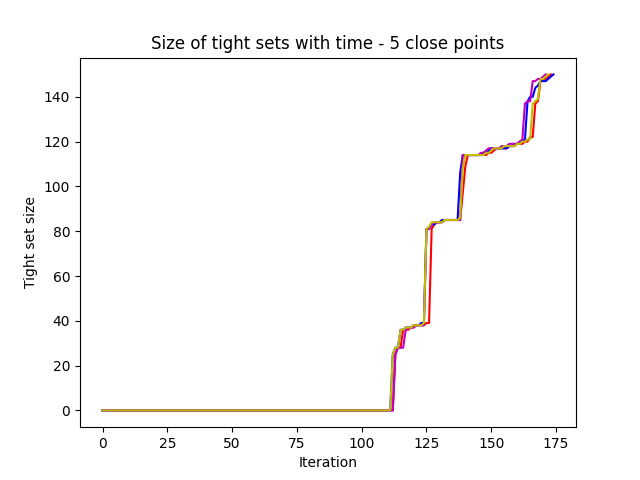
\includegraphics[width=0.43\textwidth]{code/figures/close-points/150-5-close-points-tight-sets.png}
    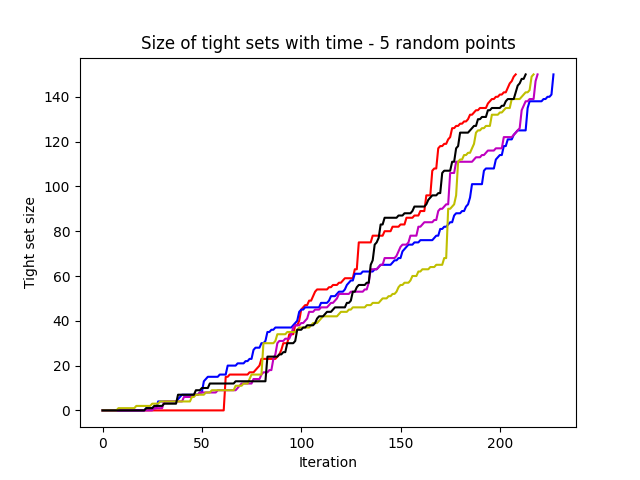
\includegraphics[width=0.43\textwidth]{code/figures/random-points/150-5-random-points-tight-sets.png}
    \caption{Size of tight sets as a function of number of iterations for (i) $5$ close points (ii) $5$ randomly generated points for $n = 150$. Clearly, tight sets follow each other closely for close points. The curves in (i) are not only close, but roughly similar in shape, which indicates that the same coordinates become tight in this case. Figures for varying $n$ can be found in \texttt{code/figures/close-points} and \texttt{code/figures/random-points} respectively.}
    \label{tight-sets-sizes-with-iteration}
\end{figure}

\begin{figure}
    \centering
    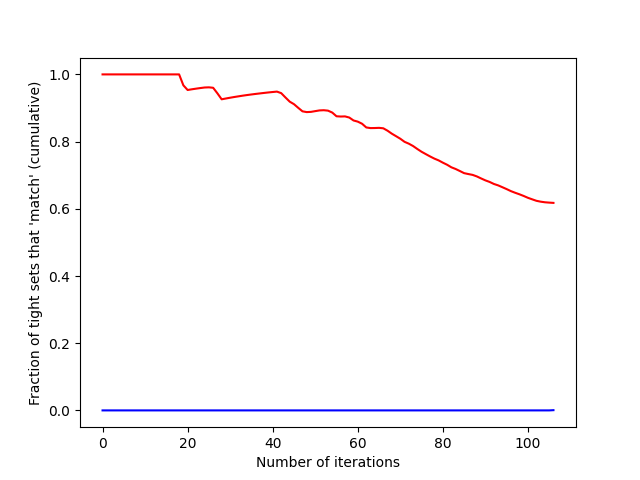
\includegraphics[width=0.43\textwidth]{code/figures/tight-set-matches/absolute-75.png}
    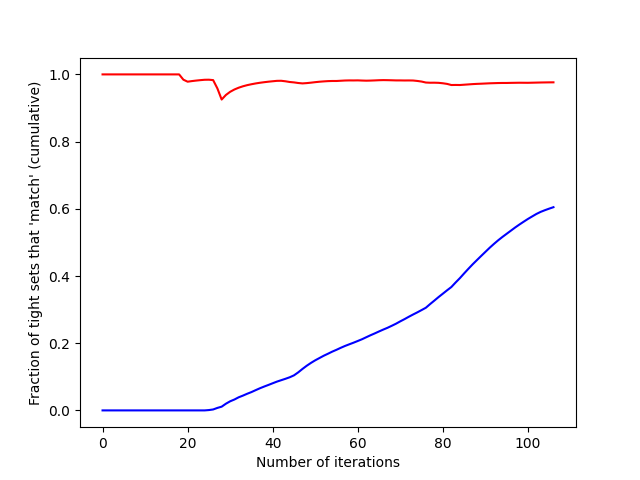
\includegraphics[width=0.43\textwidth]{code/figures/tight-set-matches/75.png}
    \caption{Fraction of tight sets that `match' (cumulatively) after each iteration of inc-fix for close points (red) and random points (blue), averaged over 100 points. Match is defined in $2$ different ways: (i) Two sets match if they are equal, and (ii) Two sets $A, B$ have fractional match $\frac{2 \times |A \cap B|}{|A| + |B|}$, assuming one of $A, B$ is nonempty. $n = 75$.}
    \label{fig:tight-set-matches-vs-iteration}
\end{figure}

\begin{figure}
    \centering
    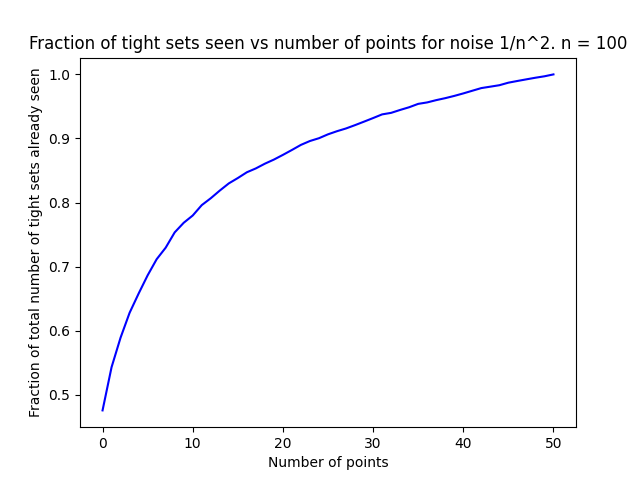
\includegraphics[width=0.43\textwidth]{code/figures/n=100-fraction-of-tight-sets-seen-noise-1-by-n^2.png}
    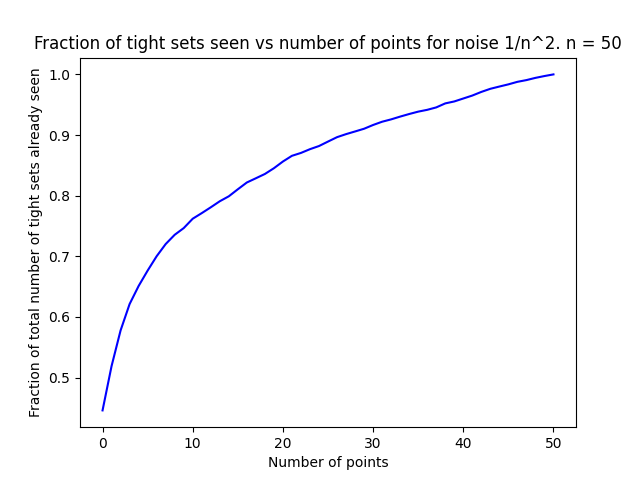
\includegraphics[width=0.43\textwidth]{code/figures/n=50-fraction-of-tight-sets-seen-noise-1-by-n^2.png}
    \caption{Fraction of unique tight sets already seen after running inc-fix on $x$ points. The $x$-coordinates represents the number of points on which inc-fix is run. The corresponding $y$-coordinates are the number of unique tight sets seen upto that point divided by the total number of unique tight sets for all points. Figure (i) is for $n = 100$ and (ii) for $n = 50$. The noise in the definition of close points is $1/n^2$ here. Roughly $70-80 \%$ unique tight sets are seen in the first $10$ points out of a total of $50$ points.}
    \label{fig:my_label}
\end{figure}

\begin{figure}
    \centering
    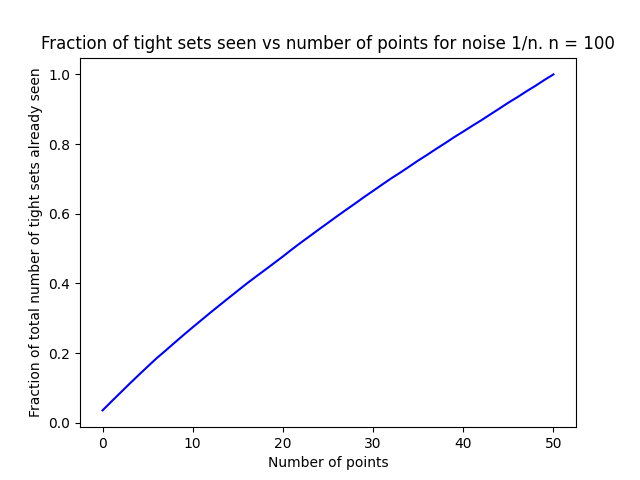
\includegraphics[width=0.43\textwidth]{code/figures/n=100-fraction-of-tight-sets-seen-noise-1-by-n.png}
    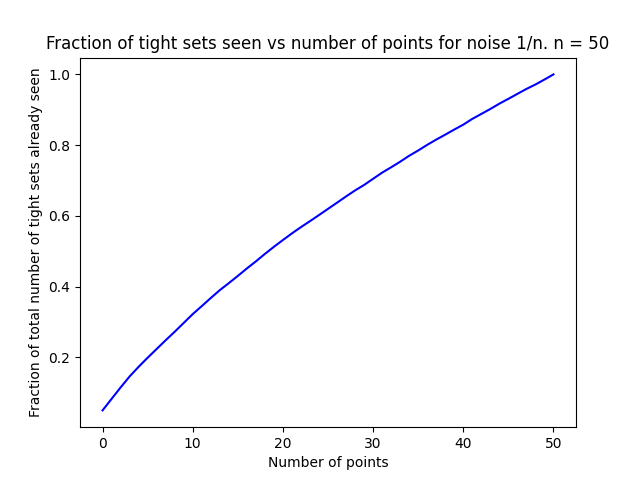
\includegraphics[width=0.43\textwidth]{code/figures/n=50-fraction-of-tight-sets-seen-noise-1-by-n.png}
    \caption{Fraction of unique tight sets already seen after running inc-fix on $x$ points, for noise $1/n$. This tells us that making the noise even as large as $1/n$ -- note that the average disturbance is $1/n$ in each coordinate in this case.}
    \label{fig:my_label}
\end{figure}

\newpage
\subsection*{Questions}

\begin{itemize}
    \item What happens if two `close' points $x, y$ differ only on one coordinate? What if this is the first coordinate w.r.t $x$? (That is, first coordinate when $x$ is sorted in decreasing order.) To make it even simpler, what happens if it is the first coordinate w.r.t both $x$ and $y$?
\end{itemize}

\newpage

\section*{Learning from Projections on (Submodular) Polytopes}
Given a ground set $E$ (with $|E|=n$) of elements, we assume the set function $f: 2^n \to \mathbb{R}$ is submodular. We will also assume throughout that the submodular function $f$ is normalized at $\emptyset$, i.e., $f(\emptyset)=0$, and is monotone non-decreasing: $f(A) \leq f(B)$ for $A \subseteq B \subseteq E$. With the empty set normalized, we know that the following polytopes are non-empty: the submodular polytope $P(f) = \{x \in \mathbb{R}_+^n | x(S) \leq f(S)\}$, and the base polytope $B(f) = \{x \in P(f) | x(E) = f(E)\}$. We consider the problem of minimizing
separable strictly convex and differentiable functions over submodular base polytopes:
\begin{equation}\label{problem}
    \min_{x \in B(f)} h(x):= \sum_{e \in E} h_e(x_e)
\end{equation}

We will use $x^*$ to denote the optimal solution of \eqref{problem}, where uniqueness follows by the strict convexity of the objective function. Let $F_1,\dots F_k$ ($k \leq n$) be partition of the ground set $E$ such that $(\nabla h(x^*))_e = c_i$ for all $e \in F_i$ and $c_i < c_j$ for $i<j$. Further, let $H_i = \{e \in E : (\nabla h(x^*))_e \leq c_i\}$ for $i= 1, \dots,k$. Then, using first-order optimality we know that $x$ is the optimal solution of problem \eqref{problem} if and only if $x(H_i) = f (H_i)$ for all $i= 1, \dots,k$.

This gives us a structural characterization of convex minimizers over submodular polytopes. Although we do not know what the optimal solution is in advance, we can exploit the combinatorial structure of the submodular polytope to construct the tight sets $H_i$ and simultaneously obtain the optimal solution, which is what the \textsc{Inc-Fix} algorithm does. We now list a few (combinatorial) properties about convex minimizers over submodular polytopes that we will be useful for our analysis.


For $\alpha \in \mathbb{R}$, define $\bar{x}_\alpha \in \mathbb{R}^n$ as
\begin{equation} \label{alpha}
    \bar{x}_\alpha = (\nabla h_e)^{-1}(\alpha) \quad \text{for all $e \in E$}.
\end{equation}
Also, let $f_\alpha: = f - \bar{x}_\alpha$ and note that $f_\alpha$ is also submodular. It is easy to see that $f_\alpha - f_{\alpha^\prime}$ is monotone non-decreasing and this relation for $\alpha < \alpha^\prime$, which we denote by $f_\alpha \to f_{\alpha^\prime}$ is called a strong map. We are now ready to list our properties.

\begin{lemma}[Nagano] \label{gradient space}
Consider $\alpha$ satisfying $c_s \leq \alpha < c_{s+1}$. If $ \alpha > c_s$, then $H_s$ is the unique minimizer of $f_\alpha$. If $ \alpha = c_s$, then $H_{s-1}$ is the unique minimal minimizer and $H_s$ is the unique maximal minimizer of $f_\alpha$.
\end{lemma}

\begin{proof}
Suppose $c_s < \alpha < c_{s+1}$. Then  as $h^\prime$ is strictly increasing, $x^*(e) - \bar{x}_\alpha(e) < 0$ if $e \in H_s$ and $x^*(e) - \bar{x}_\alpha(e) > 0$ otherwise. Recall that Using first-order optimality we know that $x^*(H_s) = f(H_s)$. Thus for any $X  \subseteq E$ with $X\neq H_s$ we have
\begin{align*}
    f_\alpha (X)  &= f(X) - \bar{x}_\alpha(X) \geq x^*(X) - \bar{x}_\alpha(X)\\
    & = (x^* - \bar{x}_\alpha(X)) (H_s) +  (x^* - \bar{x}_\alpha(X))(X \setminus H_s) - (x^* - \bar{x}_\alpha(X))(H_s \setminus X)\\
    &> x^*(H_s) - \bar{x}_\alpha(H_s)\\
    &= f(H_s) - \bar{x}_\alpha(H_s) =  f_\alpha (H_s)
\end{align*}
where the first inequality uses feasibility of $x^*$ and the second inequality uses the property that $x^*(e) - \bar{x}_\alpha(e) < 0$ if $e \in H_s$ and $x^*(e) - \bar{x}_\alpha(e) > 0$ otherwise.

Now, suppose $ \alpha = c_s$ holds. Then $e \in H_{s-1}$ if and only if
$x^*(e) - \bar{x}_\alpha(e) < 0$, $e \in H_{s}$ if and only if
$x^*(e) - \bar{x}_\alpha(e) \leq 0$. So $H_{s-1}$ and $H_s$ minimize $f_\alpha$ and any minimizer $X$ satisfies $H_{s-1} \subseteq X \subseteq H_s$.
\end{proof}

The above lemma suggests that if we have a procedure to search for $\alpha$ (say by a binary search), then convex minimization over the base polytope reduces to parametric submodular function minimization:
\begin{equation}\label{prob param}
    \min_{X \subseteq E} \{f_\alpha (X)\} \quad \text{for all $\alpha$}.
\end{equation}
Moreover, By successively computing $\bar{x}_\alpha$ for some appropriately chosen $\alpha$, and minimizing the function $f_\alpha$, we find $H_s$ one by one and finally we obtain the chain $ \emptyset = H_0 \subset H_1 \subset \dots \subset H_k$ and the point $x^*$. For such an appropriately chosen strictly decreasing sequence $\{\alpha_i\}$ we know that $f_{\alpha_k} \to f_{\alpha_{k-1}} \to \dots \to f_{\alpha_1}$. Therefore, the maximal minimizer $S_i$ of $f_{\alpha_i}$ contains in the maximal minimizer $S_j$ of $f_{\alpha_j}$ for $\alpha_i > \alpha_j$ and so this bounds the number of iterations of those paramtetric submodular function minimizations $k$ by the size $n$ of the ground set.

Let us now continue our exposition with more properties. Suppose that we are given two subsets $S = H_s$ and $T = H_t$ for some $s$ and
$t$ such that $0 \leq s < t \leq k$. For example, we know that $E$ and $\emptyset$ are always tight for any point (including $x^*$) in the base polytope. Let $\alpha$ be the parameter satisfying 
\begin{equation*}
    \bar{x}_\alpha (T \setminus S) = f (T ) - f (S)
\end{equation*}
and let $R$ be the maximal minimizer of $f_{\alpha}$.

\begin{lemma} \label{gradient 1}
Suppose that $s + 1 = t$. Then $\alpha = c_t$ and $R=T$. In addition, $\bar{x}_\alpha(e) = x^*(e)$ for all $e \in T\setminus S$.
\end{lemma}
\begin{proof}
Since $(\nabla h(x^*))_e = c_t$ for all $e \in T\setminus S$, we have
\begin{align*}
    \bar{x}_{c_t}(T\setminus S) = \sum_{e \in T\setminus S} (\nabla h_e)^{-1}(c_t) = x^*(T \setminus S) = f(T) - f(S)
\end{align*}
and thus we have $\alpha = c_t$ and $\bar{x}_\alpha(e) = x^*(e)$ for all $e \in T\setminus S$ as claimed. Moreover, by Lemma \ref{gradient space} we have $R = H_t = T$.
\end{proof}


\begin{lemma}\label{gradient 2}
Suppose that $s + 1 < t$. Then $ c_{s+1} < \alpha < c_t$ and $S \subset R \subset T$.
\end{lemma}
\begin{proof}
Using the fact that the sets $H_s$ form a chain and $x^*(H_s) = f(H_s)$ for all $s = 1,\dots k$ we have
\begin{align*}
    \bar{x}_{\alpha}(T\setminus S) &= f(T) - f(S) = \sum_{r = s+1}^t (f(H_r) - f(H_{r-1}))  \\
    &= \sum_{r = s+1}^t x^*(H_r\setminus H_{r-1}) = \sum_{r = s+1}^t \bar{x}_{c_r}(H_r\setminus H_{r-1}).
\end{align*}
Therefore, since $c_j > c_{s+1}$ for $j > s+1$ and $h^\prime$ is strictly increasing, we have $\bar{x}_{\alpha}(T\setminus S) > \sum_{r = s+1}^t \bar{x}_{c_{s+1}}(H_r\setminus H_{r-1}) = \bar{x}_{c_{s+1}}(T\setminus S)$ and $\bar{x}_{\alpha}(T\setminus S) < \sum_{r = s+1}^t \bar{x}_{c_{t}}(H_r\setminus H_{r-1}) = \bar{x}_{c_{t}}(T\setminus S)$. So we have $\bar{x}_{c_{s+1}}(T\setminus S)< \bar{x}_{\alpha}(T\setminus S) <\bar{x}_{c_{t}}(T\setminus S)$, which implies $ c_{s+1} < \alpha < c_t$ as claimed. Moreover, by Lemma \ref{gradient space} we have $S \subset R \subset T$.
\end{proof}

By Lemmas \ref{gradient 1} and \ref{gradient 2}, the maximal minimizer $R \subseteq E$ of $f_\alpha$ satisfies $``R = T"$ or
$``S \subset R \subset T"$. 
\begin{enumerate}[(i)]
    \item Case 1: Consider the case where $R = T$ . Then it holds that $t = s + 1$ and $\bar{x}_\alpha(e) = x^*(e)$ for all $e \in T\setminus S$. In this case, a decomposition algorithm $\mathcal{D}(S, T)$ returns $x^*_{T\setminus S} = \bar{x}_\alpha(T\setminus S) = (x^*(v): v \in T \setminus S)$.
    \item Case 2: Next, let us consider the case where $S \subset R \subset T$. By Lemma \eqref{gradient space}, $R = H_r$ for some $r$ with $s + 1 \leq r < t$. {To see this note that using Lemma \ref{gradient 2}, we know that $ c_{s+1} < \alpha < c_t$. In particular, $c_{r} < \alpha < c_{r+1}$ for some $r$ with $s + 1 \leq r < t$. Now directly applying Lemma \ref{gradient space} we have that $H_r = R$ is the maximal minimizer of $f_\alpha$.} Let $x_1 = x^*_{R\setminus S}$ and $x_1 = x^*_{T\setminus R}$ be vectors returned by $\mathcal{D}(S, R)$ and $\mathcal{D}(R, T)$, respectively. The algorithm $\mathcal{D}(S, T)$ returns the vector $x^*_{T\setminus S}$ defined by $x^*_{T\setminus S}(v) = x_1(v)$ if $v \in R\setminus S$ and $x^*_{T\setminus S}(v) = x_2(v)$ if $v \in T\setminus R$ (recall that $S \subset R \subset T$ and so $T \setminus S = \{R \setminus S\} \cup \{T \setminus R\}$). By induction, we can see that $x^*_{T\setminus S} = (x^*(v): v \in T \setminus S)$.
\end{enumerate}

This is the idea of the parametric gradient search implementation of $\textsc{Inc-Fix}$. 

In particular, we can solve \eqref{problem} using $\mathcal{D}(\emptyset, E)$, since we know that both $E$ and $\emptyset$ are tight at any optimal solution. In particular, it is easy to see that the Case 1 is executed at most $n$ times in total and Case 2 is executed at most $n - 1$ times in total. Therefore, we obtain $x^*$ after solving at most $2n - 1$ submodular function
minimizations.

A natural question at this point is suppose we are trying to project two points that are ``close'' to each other, then how do the tight sets and the sequence $\{\alpha_i\}$  change? For any point $y \in \mathbb{R}^n$ and polytope $P \subseteq \mathbb{R}^n$, let $\Pi_P(y) := \argmin_{x \in P} \frac{1}{2}\| y - x\|_2^2$ be the Euclidean projection operator over $P$. Now suppose that we computed $x^* = \Pi_{B(f)}(y)$ and we know the chain of tight sets $H_s$ at that point after running $\textsc{Inc-Fix}$ or the decomposition algorithm. Suppose we want to project another point $\Tilde{y}$ that is ``close'' to $y$, can we figure out what the new tight sets are at $\tilde{x} = \Pi_{B(f)}(\Tilde{y})$?

Now, similar to before, let $\alpha$ be the parameter satisfying 
\begin{equation*}
    \bar{x}_\alpha (H_1 \setminus \emptyset) = f (H_1) - f(\emptyset)
\end{equation*}
This is equivalent to finding $\alpha$ such that $(\Tilde{y} + \alpha \mathbbm{1})(H_1) = f(H_1)$. Now if $\bar{x}_\alpha \in P(f)$ then $H_1$ is also tight set at $\tilde{x}$. Indeed, if $\bar{x}_\alpha \in P(f)$ we know that $f_\alpha$ is non-negative and monotone, which implies that $H_1$ is a minimizer of \eqref{prob param}. Now, by Lemma \ref{gradient space} it follows that $H_1$ is also tight at $\tilde{x}$. However it is unclear whether $H_1$ is also the first tight set at $\tilde{x}$ or there is a smaller set $\tilde{H} \subset H_1 $ is also tight. 

Can we reverse engineer the notion of closeness so that $\bar{x}_\alpha \in P(f)$. Can we use that same approach to construct the other tight sets

Some more results:
\begin{lemma}
    If $\overline{x}_\alpha \in P(f)$, then $\overline{x}_\alpha(e) \le x^*(e)$ for all $e \in E$.
\end{lemma}

\begin{proof}
    If $\alpha \le c_1$, then for each $e \in E$, 
    \[
        x^*(e) = \big((h_e^\prime)^{-1} \circ h_e^\prime \big)(x^*(e)) = \big((h_e^\prime)^{-1}\big)(c_i) \ge \big((h_e^\prime)^{-1}\big)(\alpha) = \overline{x}_\alpha(e).
    \]
    The first inequality follows because $(h_e)^{-1}$ is strictly increasing and $c_i \ge c_1 \ge \alpha$. If $\alpha > c_1$, then 
    \[
        \overline{x}_\alpha(H_1) = \sum_{e \in H_1} \overline{x}_\alpha(e) = \sum_{e \in H_1} \big(h_e^\prime\big)^{-1}(\alpha) > \sum_{e \in H_1} \big(h_e^\prime\big)^{-1}(c_1) = \sum_{e \in H_1} x^*(e) = f(H_1),
    \]
    which is a contradiction since $\overline{x}_\alpha$ is feasible.
\end{proof}

\newpage

\subsection*{Learning over Projections forming a line}
We start by exploiting the case when the points we want to project lie on a line segment. For any point $y \in \mathbb{R}^n$ and polytope $P \subseteq \mathbb{R}^n$, let $\Pi_P(y) := \argmin_{x \in P} \frac{1}{2}\| y - x\|_2^2$ be the Euclidean projection operator over $P$. Moreover, for any $x \in P$, let $N_P(x)$ be the normal cone at $x$. From first order optimality we know that
$$z = \Pi_P(y) \quad \Leftrightarrow \quad y - z \in N_P(z).$$


\begin{lemma}
Let $P \subseteq \mathbb{R}^n$ be a polytope and let $y_1,y_2 \in \mathbb{R}^n$ be arbitrary. Further, let $z_1 =\Pi_P(y_1)$ and $z_2 =\Pi_P(y_2)$ and suppose that $N_P(z_1) = N_P(z_2)$. Then,
$$ \Pi_P( \delta y_1 + (1 - \delta) y_2) = \delta z_1 + (1 - \delta) z_2 \quad \text{for any $\delta \in [0,1]$}.$$
\end{lemma}

The proof tracks the proof of Lemma 2 in the Walking in The Shadow paper.

\begin{proof}
We will show that $\delta z_1 + (1 - \delta) z_2$ satsifies the first-order optimality condition for $\Pi_P( \delta y_1 + (1 - \delta) y_2)$. First, the first-order optimality condition for $z_1$ implies that
\begin{equation}\label{lemma eq1}
    y_1 - z_1 \in N_P(z_1).
\end{equation}
Similarly, the first-order optimality condition for $z_2$ implies that
\begin{equation}\label{lemma eq2}
    y_2 - z_2 \in N_P(z_2).
\end{equation}

Aggregate equations \eqref{lemma eq1} and \eqref{lemma eq2} with weights $\delta$ and $(1 - \delta)$ respectively to obtain:
\begin{equation}\label{lemma eq3}
    \delta y_1 + (1 - \delta) y_2 - (\delta z_1 + (1 - \delta) z_2) \in \delta N_P(z_1) + (1- \delta) N_P(z_2).
\end{equation}

Now we claim that 
\begin{equation}\label{eq4 - lemma}
        \delta N_P(z_1) + (1 - \delta) N_P(z_2) = N_P(\delta z_1 + (1 - \delta) z_2).
\end{equation}
Assuming this claim, we can write \eqref{lemma eq3} as 
\begin{equation*}
    \delta y_1 + (1 - \delta) y_2 - (\delta z_1 + (1 - \delta) z_2) \in N_P(\delta z_1 + (1 - \delta) z_2),
\end{equation*}
which shows that $\delta z_1 + (1 - \delta) z_2$ satsifies the first-order optimality condition for $\Pi_P( \delta y_1 + (1 - \delta) y_2)$. The proof of the claim \eqref{eq4 - lemma} could be found in the proof of Lemma 2 in the Walking in The Shadow paper.
\end{proof}

\end{document}
